\documentclass[a4paper,10pt]{jsarticle}

% レイアウト
\setlength{\textwidth}{\fullwidth}
\setlength{\textheight}{39\baselineskip}
\addtolength{\textheight}{\topskip}
\setlength{\voffset}{-0.5in}
\setlength{\headsep}{0.3in}
\pagestyle{myheadings}

% パッケージ
\usepackage[dvipdfmx]{graphicx}
\usepackage{amsmath,amssymb,epsfig}
\usepackage{bm}
\usepackage{ascmac}
\usepackage{pifont}
\usepackage{multirow}
\usepackage{enumerate}
\usepackage{cases}
\usepackage{type1cm}
\usepackage{cancel}
\usepackage{url}
\usepackage{listings,jlisting}
% 大きな中括弧
\usepackage{cases}

% 定義
\DeclareMathOperator*{\argmin}{arg\,min}
\DeclareMathOperator*{\argmax}{arg\,max}
\def\vec#1{\mbox{\boldmath$#1$}}
\def\R{{\Bbb R}}

% カウンタの設定
\setcounter{section}{0}
\setcounter{subsection}{0}
\setcounter{subsubsection}{0}
\setcounter{equation}{0}

% キャプションの図をFigに変更
\renewcommand{\figurename}{Fig.}
\renewcommand{\tablename}{Tab.}

% 式番号を式(章番号.番号)に
\makeatletter
\renewcommand{\theequation}{\arabic{section}.\arabic{equation}}
\@addtoreset{equation}{section}
\makeatother

% 表紙
\title{知能システム学特論レポート}
\author{
(DL2班)Caffe on Ubuntu\\
}
\date{2015年\ 7月\ 6日}

% ドキュメントの開始
\begin{document}
\maketitle
\section{報告者}
\begin{list}{}{}
 \item 15344203\hspace{0.5cm} 有田 裕太
 \item 15344206\hspace{0.5cm} 緒形 裕太
 \item 15344209\hspace{0.5cm} 株丹 亮
 \item 12104125\hspace{0.5cm} 宮本 和
\end{list}

\section{進行状況}

\begin{itemize}
\item 理論研究
\item 畳み込みネットワークについて
\end{itemize}


\section{理論研究}
\subsection{ユニットの出力}

\subsection{パディング}
畳込みは画像にフィルタを重なり合う画素どおしの積を求めて,フィルタ全体の和を求める.
したがって画像からフィルタがはみ出すような位置に重ねることができず,画像内にフィルタ全体が収まる範囲内でフィルタを動かすと,畳込み処理を行った後の画像サイズは入力画像は小さくなる.
この様子をFig.~\ref{fig:88の入力画像を畳込み処理した場合の出力画像のサイズ縮小の様子}に示す.
\begin{figure}[ht]
  \begin{center}
    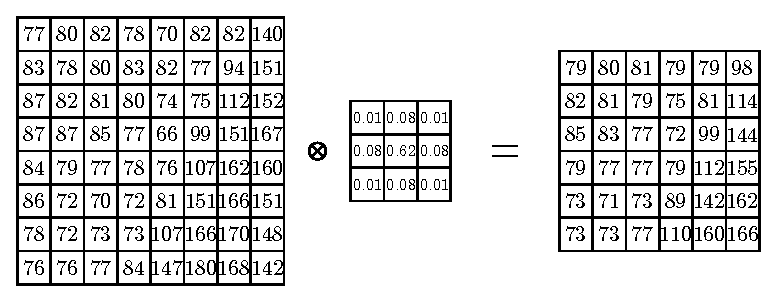
\includegraphics[clip,scale=0.8]{fig/eps/convolution.eps}
  \end{center}
  \caption{$8\times 8$の入力画像を畳込み処理した場合の出力画像のサイズ縮小の様子}
  \label{fig:88の入力画像を畳込み処理した場合の出力画像のサイズ縮小の様子}
\end{figure}

このときの画像サイズは
\begin{equation}
  \left(W-2\left\lfloor \frac{H}{2}\right\rfloor\right)\times \left(W-2\left\lfloor \frac{H}{2}\right\rfloor\right)
\end{equation}
となる.$\lfloor \cdot \rfloor$は小数点以下を切り下げて整数化する演算子である.

一方で畳込みの結果が入力画像と同サイズに出力する場合,入力画像の外側に幅$\lfloor H/2\rfloor$の余剰を設け,出力画像が元の入力画像と同サイズになるようにする.
このとき余分に設けた部分の画素値を0とする方法をゼロパディング(zero-padding)と呼ぶ.
しかしゼロパディングを行った場合,画像の周辺部が暗くなってしまうため,画像をその4辺で折り返して未定部分の画素値を決める方法や画像の最終囲の画素値をそのまま適用する方法等を用いる場合がある.
\begin{figure}[t]
  \begin{center}
    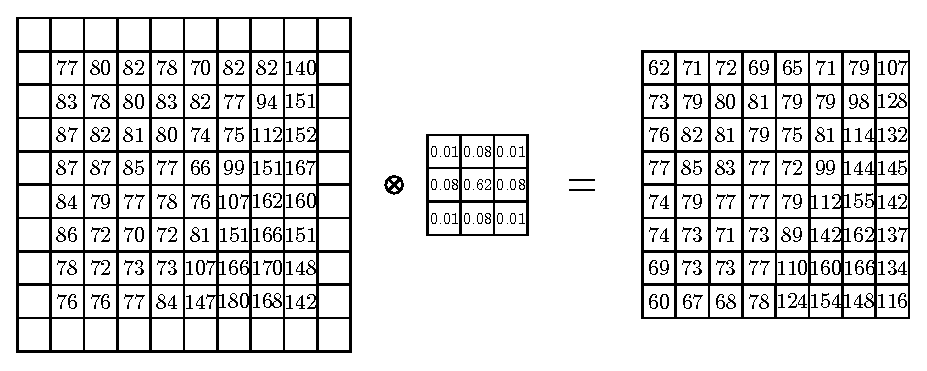
\includegraphics[clip,scale=0.8]{fig/eps/zero_padding.eps}
  \end{center}
  \caption{$8\times 8$の入力画像にゼロパディングを施した場合}
  \label{fig:88の入力画像にゼロパディングを施した場合}
\end{figure}

\subsection{ストライド}
フィルタの適用位置を1画素ずつではなく,数画素ずつずらして計算する場合がある.このずらす間隔をストライド(stride)という.ストライドを$s$とするとき,出力画像の画素値は
\begin{eqnarray}
 u_{ij} = \sum^{H-1}_{p=0}\sum^{H-1}_{q=0} x_{si+p,sj+q}h_{pq}
\end{eqnarray}
となり,出力画像のサイズは元の画像サイズの約$1/s$倍となる.サイズは正確には
\begin{eqnarray}
 \left(\left[\left(W-1\right)/s\right]+1\right)\times \left(\left[\left(W-1\right)/s\right]+1\right)
\end{eqnarray}
と計算される.

大きなサイズの入力画像を扱う際に,畳み込み層の出力側のユニット数が大きくなりすぎるのを防ぐために,2以上のストライドが使われることがある.しかし,ストライドを大きくすることは画像特徴を取りこぼすことを意味し,性能を悪化させると考えられるため,できるだけ避けるべきである.また,プーリング層においても同様の考え方が用いられる.プーリング層ではその目的から2以上のストライドを用いられる.
\section{プログラミング}
\subsection{学習を実行するPC環境の見直し}
今までcaffeのサンプル実行,中間層の出力はCPUのみの演算で十分な応答を得られた.
しかし与えられたデータセットにおいて学習を行うプログラムを実行する場合,非常に時間がかかることがわかった.

現時点では学習を行うために十分なデータ数を有するデータセットを準備できていないため,大規模なデータセットで学習済みの状態から目的とする別のデータセットへ学習し直す方法(ファインチューニング)を行った.
ファインチューニングは学習データがあまり多くない場合でも学習を行うことができる.
この手法を用いて試験的に学習用データとテスト用データを6枚ずつ用意して学習を行ったが,ファインチューニングが完全に完了するまで約3時間かかった.

このことからもこれからの課題研究を可能な限り円滑に行うために,学習時にはGPUを使った並列計算が必要であることがわかった.
したがってcaffeがサポートしているNVIDIAの「CUDA」及び,Deep Learning用のCUDAライブラリ「cuDNN」を使用する必要があると考える.
後者のライブラリはデベロッパー登録申請(CUDA Registered Developer Program)が必要であるので申請を行い,認可を待っている状態である.

\section{今後の課題}
\begin{itemize}
 \item 理論研究を進める.
 \item Caffeを使いこなす
\end{itemize}

\end{document}